\documentclass[11pt,aspectratio=169]{beamer}

% --- Packages ---
\usepackage[utf8]{inputenc}
\usepackage[vietnamese]{babel}
\usepackage{graphicx}
\usepackage{booktabs}
\usepackage{amsmath}
\usepackage{hyperref}

% --- Theme ---
\usetheme{Madrid}
\usecolortheme{whale}
\setbeamertemplate{navigation symbols}{}
\setbeamertemplate{footline}[frame number]

% --- Title ---
\title{Hệ thống Information Retrieval trên Cranfield}
\subtitle{Đánh giá và so sánh các mô hình xếp hạng}
\author{Sinh viên}
\date{\today}

\begin{document}

% ===== SLIDE 1: Title =====
\begin{frame}
\titlepage
\end{frame}

% ===== SLIDE 2: Mục tiêu =====
\begin{frame}{Mục tiêu dự án}
\begin{itemize}
    \item Xây dựng hệ thống tìm kiếm thông tin hoàn chỉnh trên bộ dữ liệu Cranfield (1400 tài liệu, 225 truy vấn).
    \item Cài đặt 4 mô hình xếp hạng: TF-IDF, BM25, QLM Jelinek-Mercer, QLM Dirichlet.
    \item Tích hợp module sửa lỗi chính tả dựa trên K-gram index và khoảng cách Levenshtein.
    \item Đánh giá hiệu suất bằng các metric tiêu chuẩn (MAP, MRR, P@K, R@K, F1@K) và tinh chỉnh siêu tham số bằng Grid Search.
\end{itemize}
\end{frame}

% ===== SLIDE 3: Kiến trúc hệ thống =====
\begin{frame}{Kiến trúc hệ thống}
\begin{columns}
\begin{column}{0.55\textwidth}
    \begin{itemize}
        \item \textbf{Backend (Python thuần)}:
        \begin{itemize}
            \item \texttt{indexer.py}: Tiền xử lý, chỉ mục ngược, K-gram index
            \item \texttt{models.py}: 4 mô hình xếp hạng
            \item \texttt{spellcheck.py}: Sửa lỗi chính tả
            \item \texttt{metrics.py}: Hàm đánh giá
        \end{itemize}
        \item \textbf{Frontend}: Streamlit (\texttt{app.py})
        \item \textbf{Notebooks}: Đánh giá và tinh chỉnh
    \end{itemize}
\end{column}
\begin{column}{0.4\textwidth}
    \small
    \begin{tabular}{l}
    \texttt{ir\_prj/} \\
    \quad \texttt{core/} \\
    \quad\quad \texttt{indexer.py} \\
    \quad\quad \texttt{models.py} \\
    \quad\quad \texttt{spellcheck.py} \\
    \quad\quad \texttt{metrics.py} \\
    \quad \texttt{notebooks/} \\
    \quad \texttt{results/} \\
    \quad \texttt{app.py} \\
    \end{tabular}
\end{column}
\end{columns}
\end{frame}

% ===== SLIDE 4: Pipeline tiền xử lý =====
\begin{frame}{Pipeline tiền xử lý văn bản}
Các bước tiền xử lý được áp dụng thống nhất cho cả tài liệu và truy vấn:
\begin{enumerate}
    \item Chuyển chữ thường (lowercase)
    \item Tách từ (tokenization) bằng biểu thức chính quy \texttt{[a-z0-9]+}
    \item Loại bỏ từ dừng (NLTK English stopwords --- 179 từ)
    \item Rút gọn gốc từ (Porter Stemmer)
\end{enumerate}
\vspace{0.5em}
Kết quả: tập từ vựng gồm khoảng 4700 term (đã stem) từ 7300 từ gốc.
\end{frame}

% ===== SLIDE 5: Kết quả đánh giá --- Bảng =====
\begin{frame}{Kết quả đánh giá --- Tham số mặc định}
\begin{table}[h]
\centering
\small
\begin{tabular}{lccccc}
\toprule
\textbf{Mô hình} & \textbf{P@10} & \textbf{R@10} & \textbf{F1@10} & \textbf{MAP} & \textbf{MRR} \\
\midrule
TF-IDF           & 0.3053 & 0.4487 & 0.3368 & 0.4097 & 0.8061 \\
BM25             & 0.3191 & 0.4573 & 0.3482 & 0.4330 & 0.8292 \\
QLM (JM)         & 0.2996 & 0.4405 & 0.3306 & 0.4061 & 0.8091 \\
QLM (Dirichlet)  & 0.2991 & 0.4359 & 0.3287 & 0.4064 & 0.8075 \\
\bottomrule
\end{tabular}
\caption{Kết quả với tham số tối ưu ($K=10$). BM25: $k_1\!=\!2.0, b\!=\!0.75$; QLM-JM: $\lambda\!=\!0.3$; QLM-Dir: $\mu\!=\!250$.}
\end{table}
\end{frame}

% ===== SLIDE 6: So sánh mô hình =====
\begin{frame}{So sánh hiệu suất các mô hình}
\begin{center}
    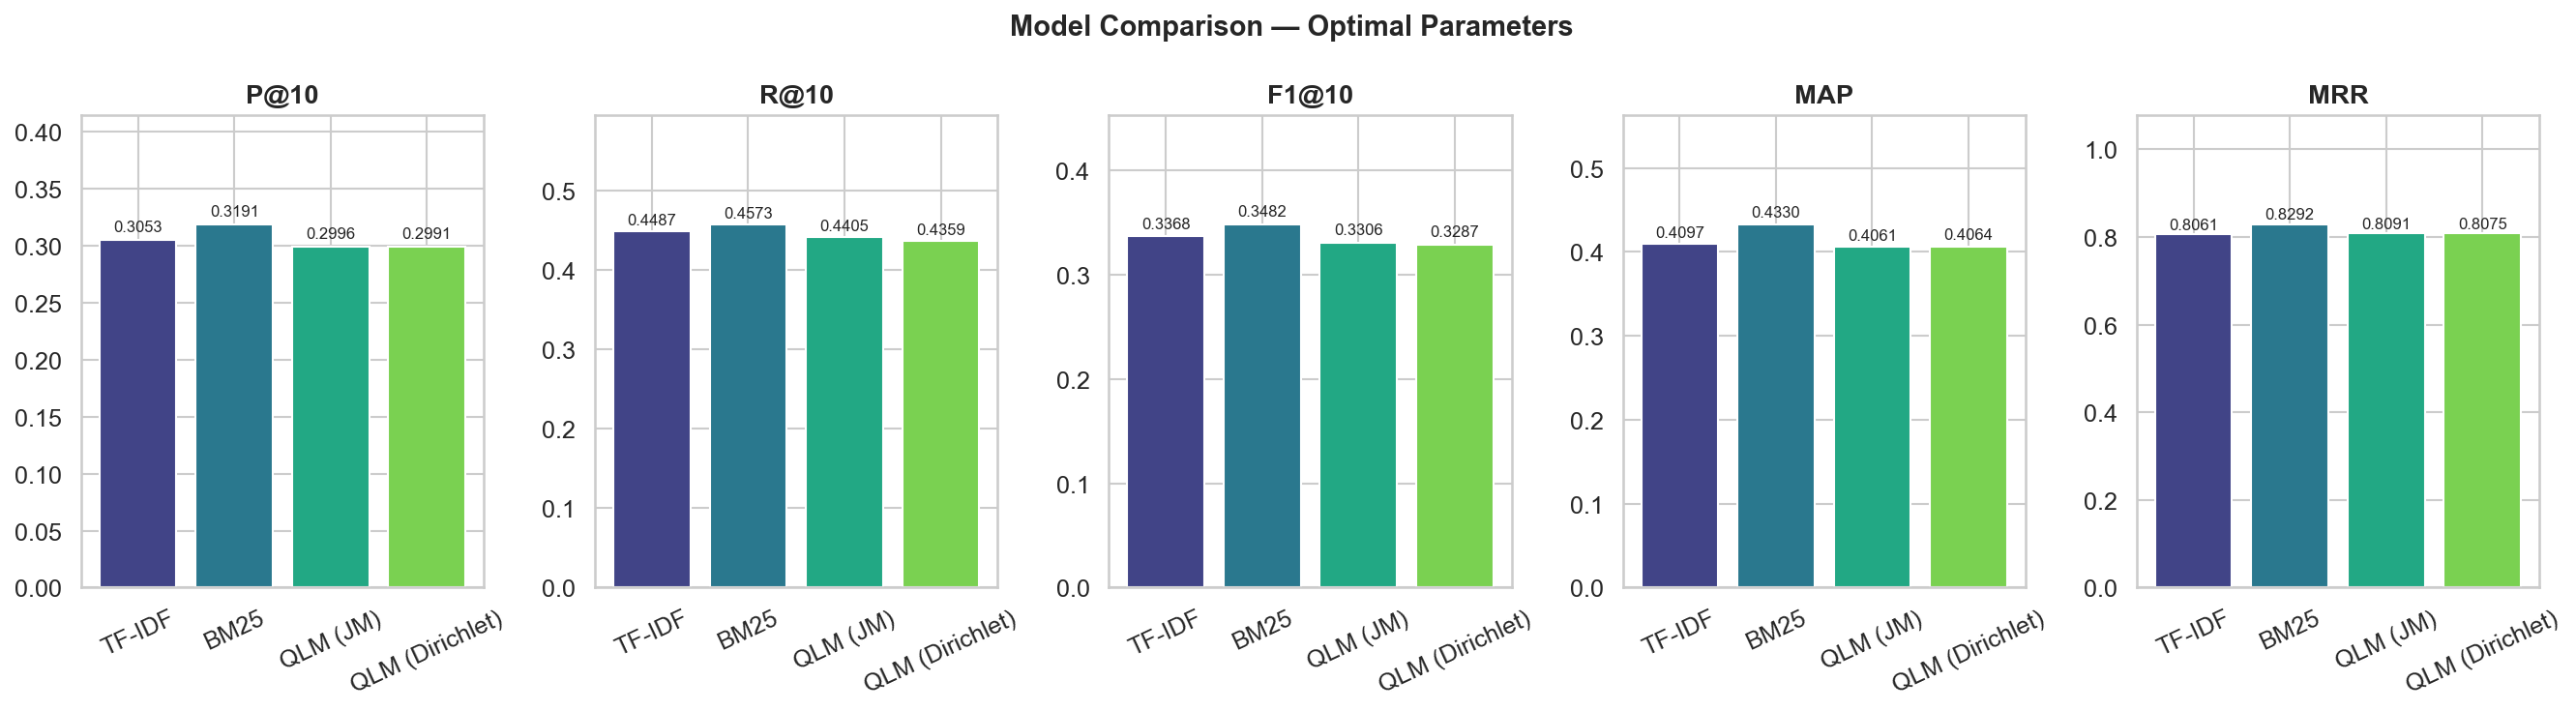
\includegraphics[width=0.85\textwidth]{figures/model_comparison_optimal.png}
\end{center}
\end{frame}

% ===== SLIDE 7: Hyperparameter Tuning --- BM25 =====
\begin{frame}{Tinh chỉnh siêu tham số --- BM25}
Grid Search trên $k_1 \in \{0.5, 0.75, 1.0, 1.2, 1.5, 2.0\}$ và $b \in \{0.25, 0.5, 0.75, 1.0\}$.
\begin{center}
    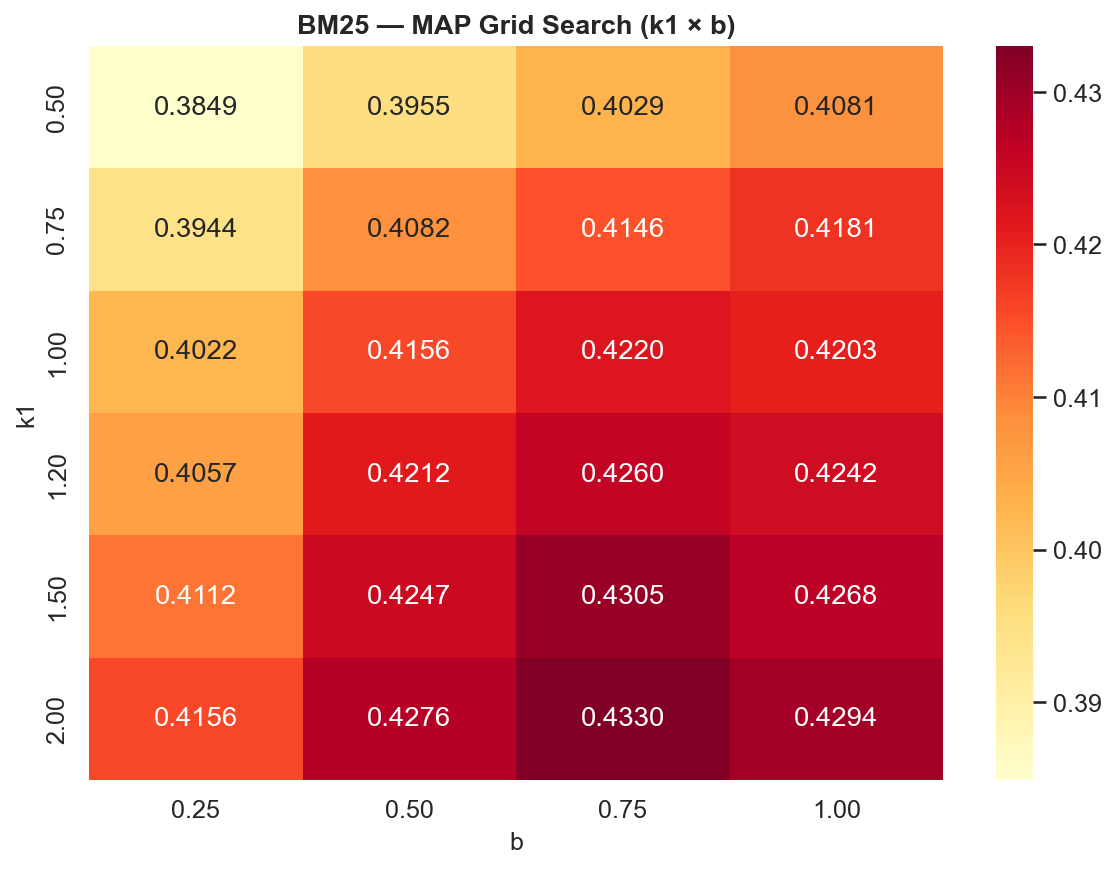
\includegraphics[width=0.65\textwidth]{figures/bm25_heatmap.png}
\end{center}
\end{frame}

% ===== SLIDE 8: Hyperparameter Tuning --- QLM =====
\begin{frame}{Tinh chỉnh siêu tham số --- QLM}
\begin{columns}
\begin{column}{0.5\textwidth}
    \centering
    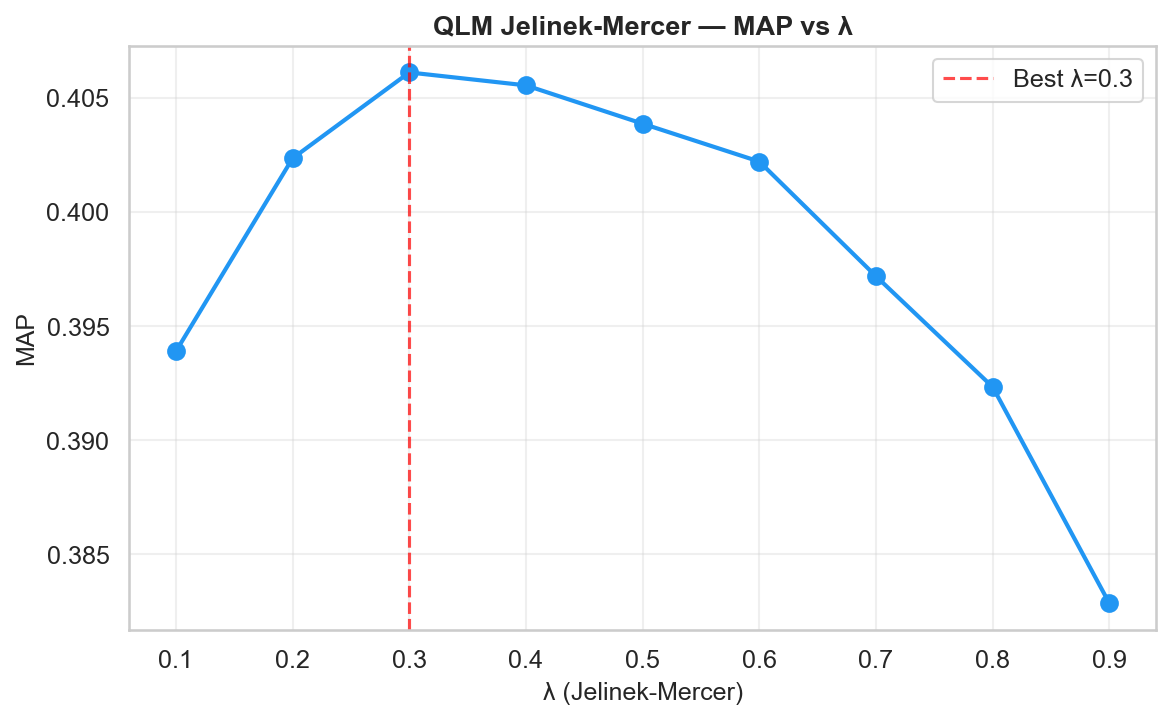
\includegraphics[width=\textwidth]{figures/qlm_jm_lambda.png}
    
    \small $\lambda$ từ 0.1 đến 0.9
\end{column}
\begin{column}{0.5\textwidth}
    \centering
    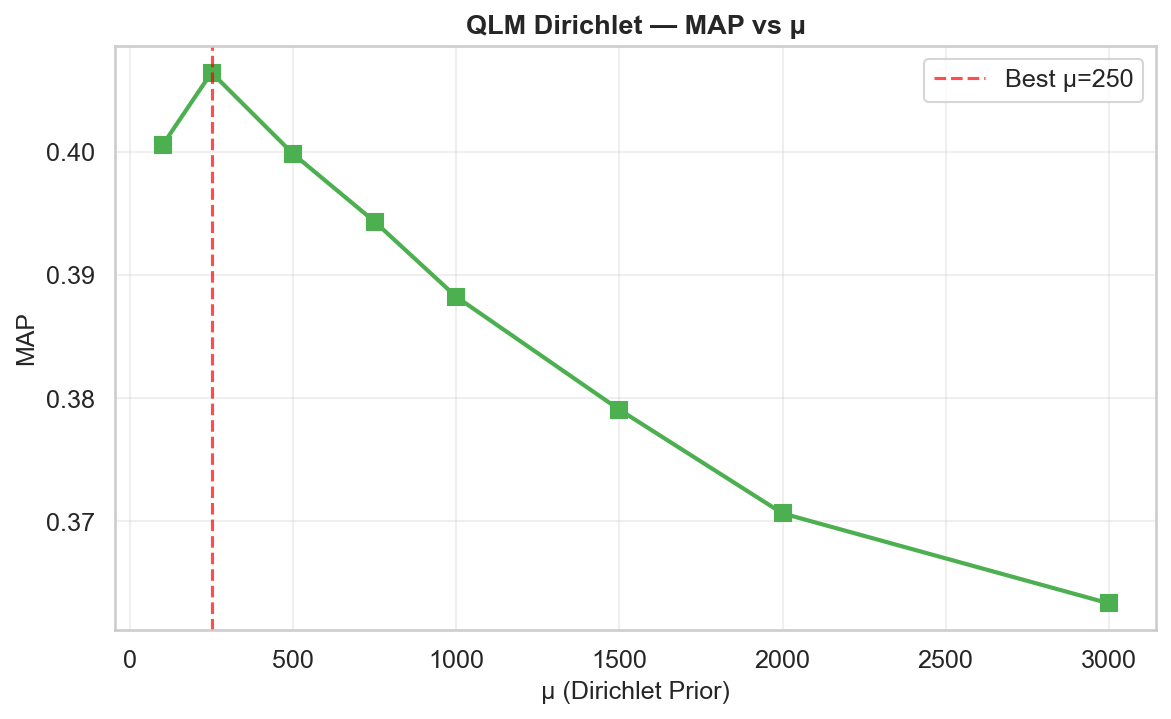
\includegraphics[width=\textwidth]{figures/qlm_dirichlet_mu.png}
    
    \small $\mu$ từ 100 đến 3000
\end{column}
\end{columns}
\end{frame}

% ===== SLIDE 9: Tolerant Retrieval =====
\begin{frame}{Tolerant Retrieval --- Sửa lỗi chính tả}
\begin{itemize}
    \item Sử dụng K-gram index (bigram) để thu hẹp tập ứng viên.
    \item Xếp hạng ứng viên bằng khoảng cách Levenshtein (edit distance).
    \item Thử nghiệm trên 10 truy vấn với lỗi chính tả cố ý.
\end{itemize}
\begin{center}
    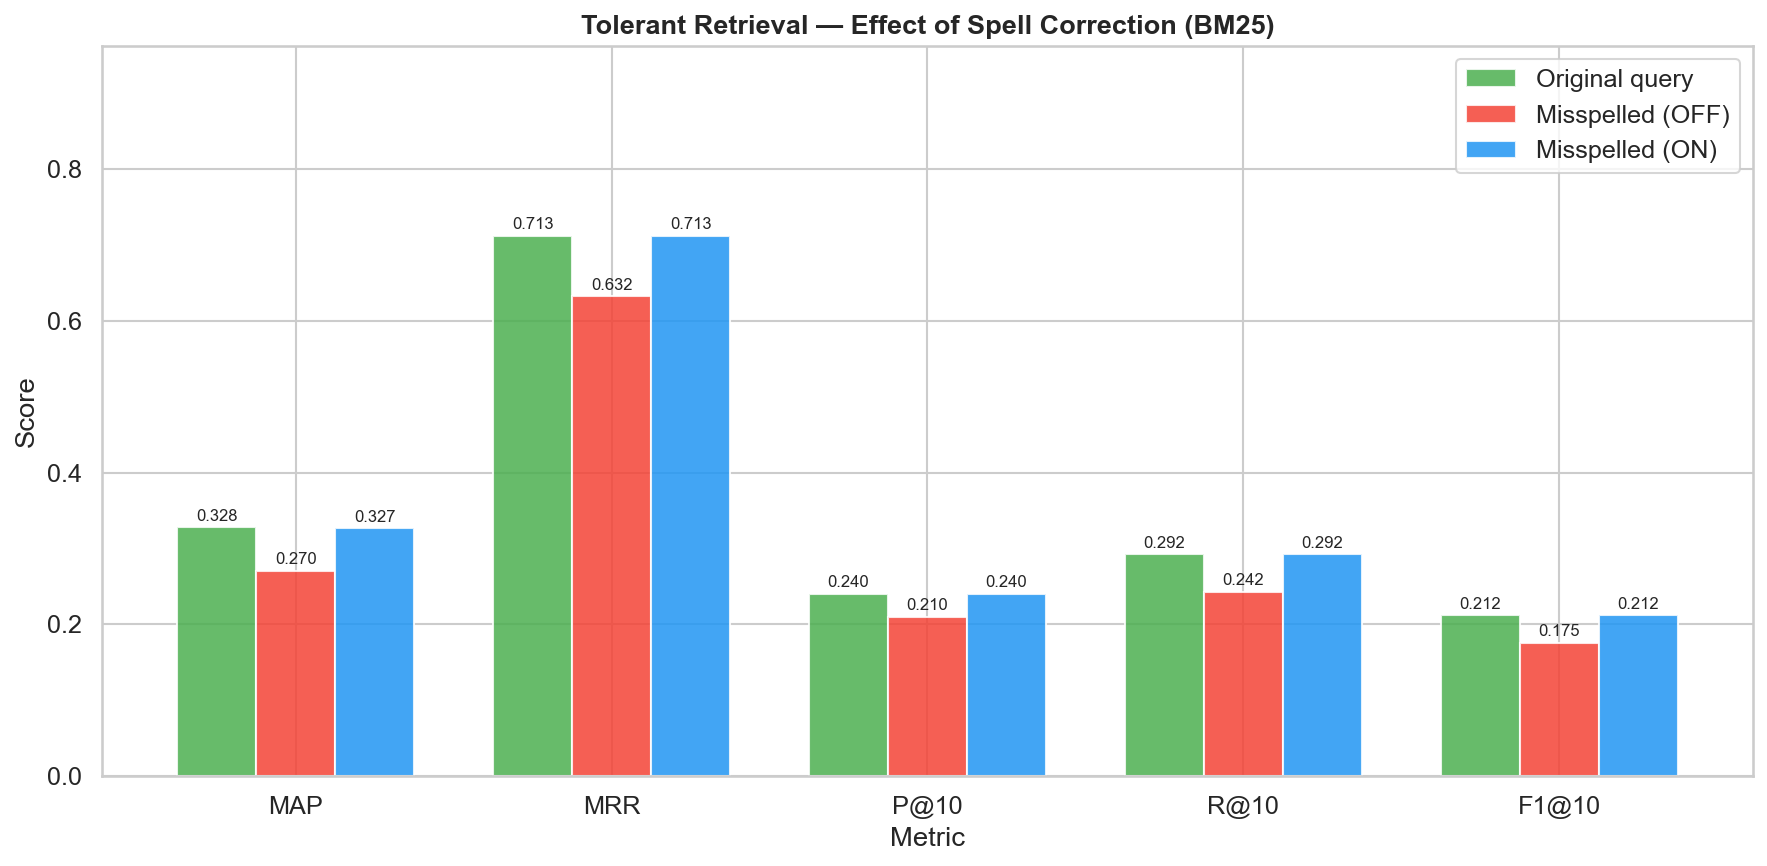
\includegraphics[width=0.7\textwidth]{figures/tolerant_comparison.png}
\end{center}
\end{frame}

% ===== SLIDE 10: Tolerant Retrieval --- Per Query =====
\begin{frame}{Tolerant Retrieval --- Phân tích theo từng truy vấn}
\begin{center}
    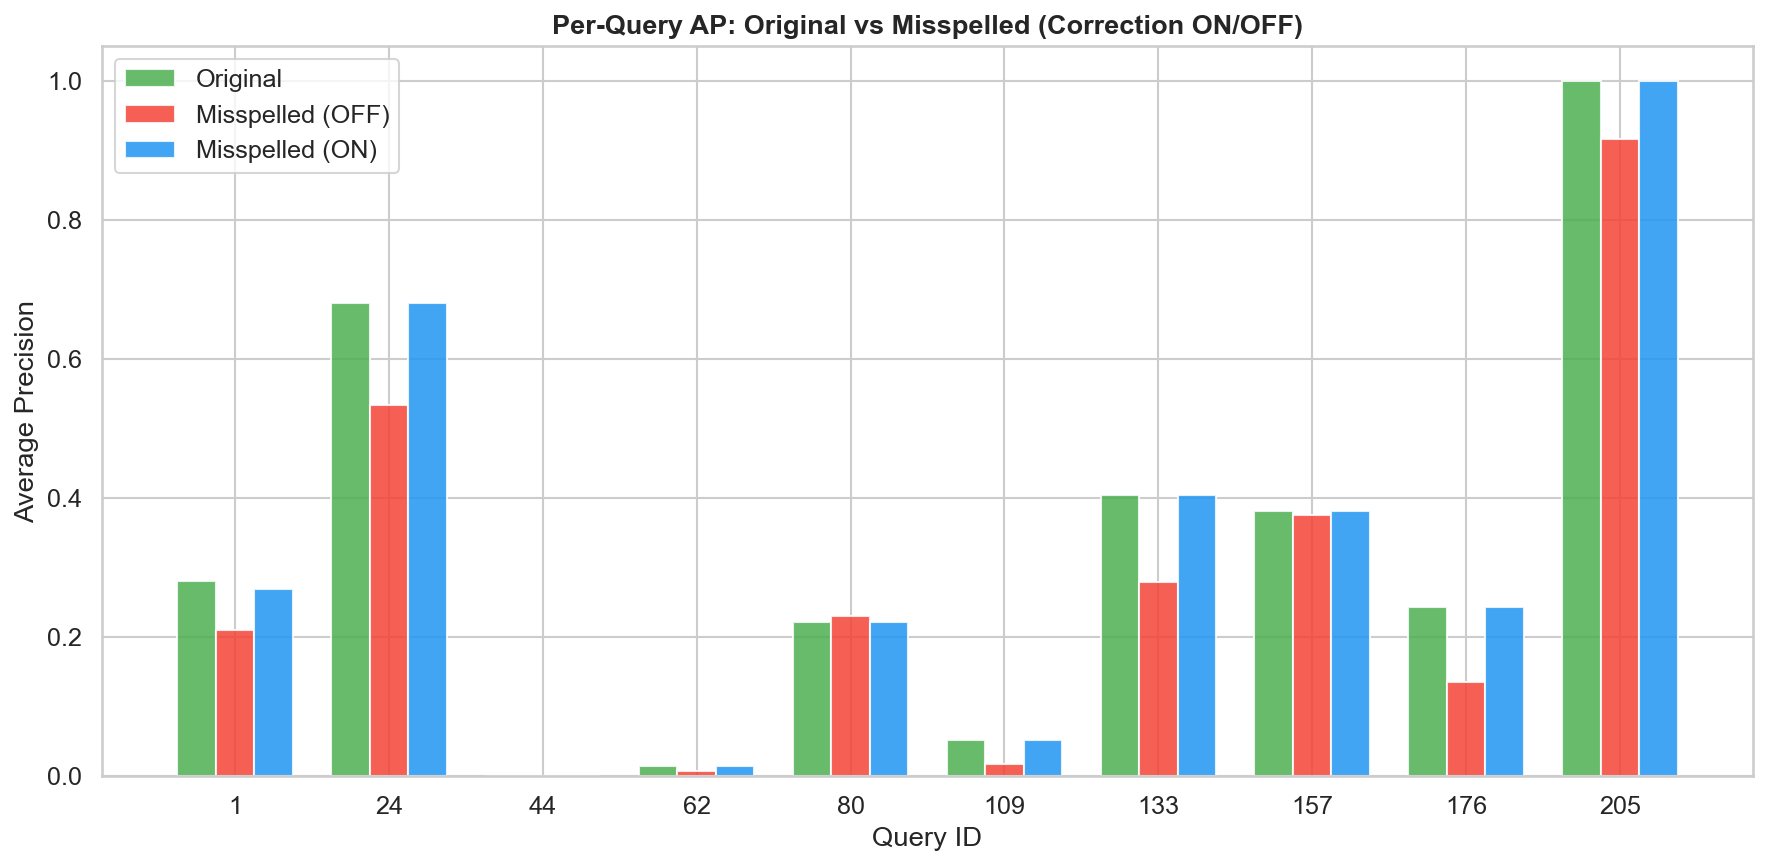
\includegraphics[width=0.8\textwidth]{figures/tolerant_per_query.png}
\end{center}
\end{frame}

% ===== SLIDE 11: Nhận xét =====
\begin{frame}{Nhận xét}
\begin{itemize}
    \item Các mô hình xác suất (BM25, QLM) cho kết quả vượt trội so với TF-IDF cơ bản.
    \item Tinh chỉnh siêu tham số cải thiện đáng kể hiệu suất, đặc biệt ở BM25.
    \item Module sửa lỗi chính tả giúp khôi phục phần lớn hiệu suất khi truy vấn bị viết sai.
    \item Pipeline tiền xử lý thống nhất đảm bảo tính nhất quán giữa đánh giá và demo.
\end{itemize}
\end{frame}

% ===== SLIDE 12: Kết luận =====
\begin{frame}{Kết luận}
\begin{itemize}
    \item Đã xây dựng thành công hệ thống IR hoàn chỉnh với 4 mô hình xếp hạng.
    \item Hệ thống có khả năng sửa lỗi chính tả và giao diện tìm kiếm trực quan.
    \item Các metric đánh giá được lập trình từ đầu, đảm bảo hiểu rõ cơ chế hoạt động.
    \item Kết quả tinh chỉnh siêu tham số được áp dụng trực tiếp vào giao diện demo.
\end{itemize}
\end{frame}

\end{document}
